\documentclass[sigconf,nonacm]{acmart}

\usepackage{enumitem}
\usepackage{graphicx}
\usepackage{hyperref}
\usepackage{tabularx}
\usepackage{float}
\usepackage[super]{nth}
\usepackage{titlesec}
\usepackage{alltt}
\usepackage{float}
\usepackage{listings}

\usepackage[utf8]{inputenc}
%% Python Source formatting
\lstset{ 
  basicstyle=\footnotesize,
  language=Python,
  frame=single
}
%%
%% \BibTeX command to typeset BibTeX logo in the docs
\AtBeginDocument{%
  \providecommand\BibTeX{{%
    \normalfont B\kern-0.5em{\scshape i\kern-0.25em b}\kern-0.8em\TeX}}}
\setlength{\parindent}{0cm}
\setlength{\parskip}{0cm}
\settopmatter{printfolios=true}

\begin{abstract}
Based on the paper
\emph{"MediaEval 2018 AcousticBrainz Genre Task: A Baseline
Combining Deep Feature Embeddings Across Datasets"}
by Oramas et al., we were working on reproducing their results on
predicting genres from different taxonomies using stacked neural
networks.

As documented in this paper we were only partially successful
in a full reproduction, mainly due to missing information in the
paper and the accompanying repository and technical issues related with
the vast amount of data to be processed.

This reproducability exercise was performed by Group 04 during
the lecture \emph{188.992 Experiment Design for Data Science}.
\end{abstract}

\renewcommand{\thesection}{\Alph{section})}
\renewcommand{\thesubsection}{(\arabic{subsection})}
\renewcommand{\thesubsubsection}{(\alph{subsubsection})}
\titleformat{\subsubsection}
  {\normalfont\bfseries}{\thesubsubsection}{1em}{}
\titleformat{\paragraph}
  {\normalfont\bfseries\itshape}{}{0em}{}
\begin{document}

%%
%% The "title" command has an optional parameter,
%% allowing the author to define a "short title" to be used in page headers.
\title{Experiment Design, Group 04 -- Reproducibility}

\subtitle{Option 2: Prediction of music genre across different taxonomies}

%%
%% The "author" command and its associated commands are used to define
%% the authors and their affiliations.
%% Of note is the shared affiliation of the first two authors, and the
%% "authornote" and "authornotemark" commands
%% used to denote shared contribution to the research.

\author{Helmuth Breitenfellner}
\email{e8725866@student.tuwien.ac.at}
\affiliation{%
}

\author{L\'aszl\'o Kir\'aly}
\email{e9227679@student.tuwien.ac.at}
\affiliation{%
}

\author{Gerald Weber}
\email{e0125536@student.tuwien.ac.at}
\affiliation{%
}

%% A "teaser" image appears between the author and affiliation
%% information and the body of the document, and typically spans the
%% page.
%\begin{teaserfigure}
%  \includegraphics[width=\textwidth]{sampleteaser}
%  \caption{Seattle Mariners at Spring Training, 2010.}
%  \Description{Enjoying the baseball game from the third-base
%  seats. Ichiro Suzuki preparing to bat.}
%  \label{fig:teaser}
%\end{teaserfigure}

%%
%% This command processes the author and affiliation and title
%% information and builds the first part of the formatted document.
\maketitle

\section{Task Description}

The original paper describes an approach of predicting music genres
as a "baseline approach" for the
\emph{MediaEval 2018 AcousticBrainz Genre Task}.

The conference provides a website for the classification
task\footnote{\url{https://multimediaeval.github.io/2018-AcousticBrainz-Genre-Task/}, seen on 2020-01-30}
which describes the task, the schedule and the dataset on a
subpage\footnote{\url{https://multimediaeval.github.io/2018-AcousticBrainz-Genre-Task/data/}, seen on 2020-01-30}
in detail.

Four classification sources ("allmusic", "discogs", "tagtraum" and "lastfm")
have genres identified for audio files, using four different taxonomies
of genres.
While the audio files themselves are not available, there is a JSON
file with precomputed audio features extracted using 
Essentia\footnote{\url{https://essentia.upf.edu/}, seen on 2020-01-30}.

Using these JSON files and one-hot encoding for the categorical
values contained,
the authors have extracted a set of 2669 features which were
then used to train a neural network per classification source.
Each network has one 256-dimensional hidden layer and the output layer,
corresponding in dimensionality with the genres used by the classification
source. 

As a follow-up step the authors have then stacked the hidden
layer representation of songs based on the four networks into
one 1024-dimensional feature vector, which is then used to predict
the genre per classification source.

As a preparational step the training data was split into 80\%/20\%
"train-train" and "train-test" data by the authors,
used for validation during the training step.

\subsection{Data Sets}

We downloaded the datasets provided by the authors via zenodo,
in addition to the "allmusic" dataset from TUWEL
(which is under a more restricted license and therefore not
publicly available).

The ground truth is provided for 4019812 entries (most songs are
classified by more than one classification source) as TSV-files.

Originally we also downloaded the test dataset.
However since there is no "ground truth" available for them, predicting
their genres without being able to validate the correctness is of
no value for us.
Therefore we removed them later on.

Overall we had to download data in the volume of (uncompressed)
more than 100GB,
split into 1772307 single files in JSON format.

We have then randomly split the training data set into 80\%
"train-train" and 20\% "train-test" data for the following tasks.

\subsection{Feature Extraction}

The first step, which is extracting the 2669 features from the provided
JSON files, is unfortunately not documented.
We have tried contacting the main author via two email addresses,
however we did not receive any response.
This is very unfortunate as the features used presumably have a great
impact on the final results.

In our attempts to recreate these features
we were somehow lucky and found a
repository\footnote{\url{https://github.com/nikuya3/acousticbrainz-mediaeval-baseline}, seen on 2020-01-30}
which was created just a few weeks ago, containing an
attempt at creating the CSV files as needed.

This third-party repository is dealing with the 2019 iteration
of the original paper.
It was a good starting point, however a lot of
work was required to achieve preprocessed data which is
compatible with the other, provided code by the authors of the paper.

It did a good job at creating \emph{almost} the correct number
of features (2668 instead of 2669 as in the original paper),
however one of the features has a constant value of 1.
Also the encoding of the ground truth had some mistakes, and we
had to implement a one-hot encoding to match the networks.

We ended up with adding one more feature, the \emph{median}
of the \emph{beats\_loudness}.
It is missing in some observations and we are filling it with the mean
of the median for the other observations in the training dataset.
We ignored the fact that one of the features has a constant value,
hoping that the impact of one feature, given the vast amount of features,
will be neglectable.

Another issue with the code was that it performed the $z$-scaling using
the mean and standard deviation estimated from \emph{all} observations,
including data from the validation set.
We changed this to only use mean and standard deviation estimates
derived from the "train-train" dataset.

When running the conversion the runtime of this step itself was
a practical issue.
Performing the conversation took more than 48 hours on the systems
available to us.
For development purposes we have therefore used a stripped-down
version of the data.
Still, when then applying the code on the full dataset new
issues popped up, like missing values and their treatment.
Overall, this "simple" step of feature extraction into CSV
format took us multiple weeks to get it correct.

\subsection{Format Conversion}

As a next step the original code was converting the data from
CSV format into sets of files in HDF5 format, \texttt{numpy}
persisted files and again TSV files for indexes.

This code was working as provided without any major issue,
except that it was necessary using Python version 2.

\subsection{Learning the Step 1 Network}

The code for learning the first network is based on Keras
with a Theano backend.

Running the code on CPU only turned out to be completely infeasible.

Making Theano run on GPU is however not an easy task either.
Development on Theano has stopped in 
2017\footnote{\url{https://groups.google.com/forum/#!msg/theano-users/7Poq8BZutbY/rNCIfvAEAwAJ}, seen on 2020-02-04},
and using GPU acceleration
is only possible with outdated libraries and operating system drivers.

We therefore had to abandon the idea of using the existing code
for the neural network.
Since the network is rather simple in nature, reimplementing
it in another platform turned out to be super simple.
We used Pytorch where we have most experience
in achieving GPU acceleration.

\subsection{Learning the Step 2 Network}

Due to time constraints we did not manage to learn all
the networks required for step 1, which means we could not
complete the step 2 network which is based on the
stacked latent feature layers.

\section{Reproduction - Additional Repository}\label{reproduction2}

Some online research led us to a recently created Github repository\footnote{\url{https://github.com/nikuya3/acousticbrainz-mediaeval-baseline}, seen on 2020-01-30} which deals with the same paper. Additionally it has a preprocessing step included. Naturally, we cloned the repository and started inspecting \textit{preprocessing.py}. The script describes the creation of the files as we described it as input for the original paper repository in  section \ref{reproduction1}.

\subsection{Datasets}

With the code from Section \ref{reproduction2} we provided the dataset according to the script and started preprocessing, which consists of 3 steps:
\begin{itemize}
  \item creating CSV feature file and a genres file per dataset
  \item calculating the mean and standard deviation of each dataset
  \item scaling each dataset
\end{itemize}
The output of the steps is written into \textit{processed} folder.
Even though the repository is very new and seems to handle the missing preprocessing step, an error occured in step 3:

\begin{lstlisting}
Preprocessing train mode of allmusic dataset
Preprocessing validation mode of allmusic dataset
Preprocessing train mode of tagtraum dataset
Preprocessing validation mode of tagtraum dataset
Preprocessing train mode of discogs dataset
Preprocessing validation mode of discogs dataset
Preprocessing train mode of lastfm dataset
Preprocessing validation mode of lastfm dataset
Finished first preprocessing pass
Calculated means and standard deviations
Scale preprocessed datasets
Scaling processed/train/allmusic
Traceback (most recent call last):
...
ValueError: Unable to coerce to Series, 
  length must be 2668: given 2669
\end{lstlisting}

Therefore \textit{preprocessing.py} has been adapted. The idea is to use the preprocessing step of the second repository to generate the files for the data-preparation step of the original repository. Afterwards the training should have all required files to start (see figure \ref{fig:preprocess}).

\subsection{Preprocessing}
  \begin{figure}
    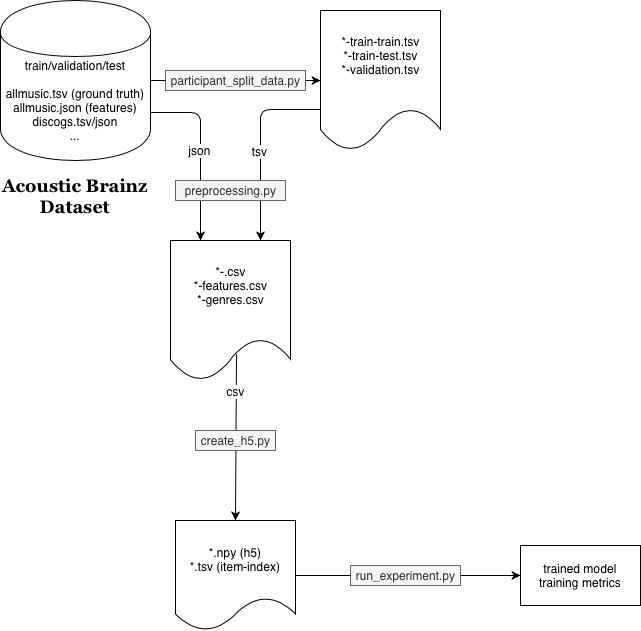
\includegraphics[width=\linewidth]{Preprocess-Data.png}
    \caption{Preprocessing Data.}
    \label{fig:preprocess}
  \end{figure}

  \begin{itemize}
    \item preprocessing.py python3
    \item participant\_split\_data.py
    \item create\_h5.py python2 with h5py
  \end{itemize}

  Problems:
  \begin{itemize}
    \item TypeError: No conversion path for dtype: dtype('<U38') https://github.com/h5py/h5py/issues/1131 -> solved with using python2
  \end{itemize}

\subsection{Train}

all python3

\begin{itemize}
  \item python run\_experiments.py genre\_allmusic
  \item python run\_experiments.py genres\_discogs
  \item ... 
  \item python run\_experiments.py genres\_allmusic\_multimodal part of our Reproducibility run???
\end{itemize}

Problems:
\begin{itemize}
  \item ValueError: Error when checking target: expected dense\_5 to have shape (766,) but got array with shape (1,)
\end{itemize}

\subsection{GPU}

Problems:

\begin{itemize}
  \item Without GPU one Epoch with only few 100 items takes hours
  \item cuda on windows 10 fails: https://github.com/Theano/libgpuarray/issues/587
\end{itemize}

\subsection{Sources}

\subsection{Doing}




\bibliography{bibliography}
\bibliographystyle{alpha}

\end{document}
\endinput
